\documentclass[twoside]{book}

% Packages required by doxygen
\usepackage{fixltx2e}
\usepackage{calc}
\usepackage{doxygen}
\usepackage[export]{adjustbox} % also loads graphicx
\usepackage{graphicx}
\usepackage[utf8]{inputenc}
\usepackage{makeidx}
\usepackage{multicol}
\usepackage{multirow}
\PassOptionsToPackage{warn}{textcomp}
\usepackage{textcomp}
\usepackage[nointegrals]{wasysym}
\usepackage[table]{xcolor}

% Font selection
\usepackage[T1]{fontenc}
\usepackage[scaled=.90]{helvet}
\usepackage{courier}
\usepackage{amssymb}
\usepackage{sectsty}
\renewcommand{\familydefault}{\sfdefault}
\allsectionsfont{%
  \fontseries{bc}\selectfont%
  \color{darkgray}%
}
\renewcommand{\DoxyLabelFont}{%
  \fontseries{bc}\selectfont%
  \color{darkgray}%
}
\newcommand{\+}{\discretionary{\mbox{\scriptsize$\hookleftarrow$}}{}{}}

% Page & text layout
\usepackage{geometry}
\geometry{%
  a4paper,%
  top=2.5cm,%
  bottom=2.5cm,%
  left=2.5cm,%
  right=2.5cm%
}
\tolerance=750
\hfuzz=15pt
\hbadness=750
\setlength{\emergencystretch}{15pt}
\setlength{\parindent}{0cm}
\setlength{\parskip}{3ex plus 2ex minus 2ex}
\makeatletter
\renewcommand{\paragraph}{%
  \@startsection{paragraph}{4}{0ex}{-1.0ex}{1.0ex}{%
    \normalfont\normalsize\bfseries\SS@parafont%
  }%
}
\renewcommand{\subparagraph}{%
  \@startsection{subparagraph}{5}{0ex}{-1.0ex}{1.0ex}{%
    \normalfont\normalsize\bfseries\SS@subparafont%
  }%
}
\makeatother

% Headers & footers
\usepackage{fancyhdr}
\pagestyle{fancyplain}
\fancyhead[LE]{\fancyplain{}{\bfseries\thepage}}
\fancyhead[CE]{\fancyplain{}{}}
\fancyhead[RE]{\fancyplain{}{\bfseries\leftmark}}
\fancyhead[LO]{\fancyplain{}{\bfseries\rightmark}}
\fancyhead[CO]{\fancyplain{}{}}
\fancyhead[RO]{\fancyplain{}{\bfseries\thepage}}
\fancyfoot[LE]{\fancyplain{}{}}
\fancyfoot[CE]{\fancyplain{}{}}
\fancyfoot[RE]{\fancyplain{}{\bfseries\scriptsize Generated by Doxygen }}
\fancyfoot[LO]{\fancyplain{}{\bfseries\scriptsize Generated by Doxygen }}
\fancyfoot[CO]{\fancyplain{}{}}
\fancyfoot[RO]{\fancyplain{}{}}
\renewcommand{\footrulewidth}{0.4pt}
\renewcommand{\chaptermark}[1]{%
  \markboth{#1}{}%
}
\renewcommand{\sectionmark}[1]{%
  \markright{\thesection\ #1}%
}

% Indices & bibliography
\usepackage{natbib}
\usepackage[titles]{tocloft}
\setcounter{tocdepth}{3}
\setcounter{secnumdepth}{5}
\makeindex

% Hyperlinks (required, but should be loaded last)
\usepackage{ifpdf}
\ifpdf
  \usepackage[pdftex,pagebackref=true]{hyperref}
\else
  \usepackage[ps2pdf,pagebackref=true]{hyperref}
\fi
\hypersetup{%
  colorlinks=true,%
  linkcolor=blue,%
  citecolor=blue,%
  unicode%
}

% Custom commands
\newcommand{\clearemptydoublepage}{%
  \newpage{\pagestyle{empty}\cleardoublepage}%
}

\usepackage{caption}
\captionsetup{labelsep=space,justification=centering,font={bf},singlelinecheck=off,skip=4pt,position=top}

%===== C O N T E N T S =====

\begin{document}

% Titlepage & ToC
\hypersetup{pageanchor=false,
             bookmarksnumbered=true,
             pdfencoding=unicode
            }
\pagenumbering{roman}
\begin{titlepage}
\vspace*{7cm}
\begin{center}%
{\Large My Project }\\
\vspace*{1cm}
{\large Generated by Doxygen 1.8.11}\\
\end{center}
\end{titlepage}
\clearemptydoublepage
\tableofcontents
\clearemptydoublepage
\pagenumbering{arabic}
\hypersetup{pageanchor=true}

%--- Begin generated contents ---
\chapter{File Index}
\section{File List}
Here is a list of all files with brief descriptions\+:\begin{DoxyCompactList}
\item\contentsline{section}{\hyperlink{Lab1_8c}{Lab1.\+c} }{\pageref{Lab1_8c}}{}
\end{DoxyCompactList}

\chapter{File Documentation}
\hypertarget{BinarySearch_8cpp}{}\section{Binary\+Search.\+cpp File Reference}
\label{BinarySearch_8cpp}\index{Binary\+Search.\+cpp@{Binary\+Search.\+cpp}}
{\ttfamily \#include $<$iostream$>$}\\*
Include dependency graph for Binary\+Search.\+cpp\+:
\nopagebreak
\begin{figure}[H]
\begin{center}
\leavevmode
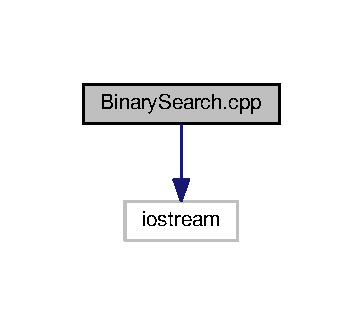
\includegraphics[width=174pt]{BinarySearch_8cpp__incl}
\end{center}
\end{figure}
\subsection*{Functions}
\begin{DoxyCompactItemize}
\item 
bool \hyperlink{BinarySearch_8cpp_a1bb2d59e960be5b8d354d92296ed9af2}{binary\+Search} (int a\mbox{[}$\,$\mbox{]}, int begin, int end, int element, int \&position)
\item 
int \hyperlink{BinarySearch_8cpp_ae66f6b31b5ad750f1fe042a706a4e3d4}{main} ()
\end{DoxyCompactItemize}


\subsection{Function Documentation}
\index{Binary\+Search.\+cpp@{Binary\+Search.\+cpp}!binary\+Search@{binary\+Search}}
\index{binary\+Search@{binary\+Search}!Binary\+Search.\+cpp@{Binary\+Search.\+cpp}}
\subsubsection[{\texorpdfstring{binary\+Search(int a[], int begin, int end, int element, int \&position)}{binarySearch(int a[], int begin, int end, int element, int &position)}}]{\setlength{\rightskip}{0pt plus 5cm}bool binary\+Search (
\begin{DoxyParamCaption}
\item[{int}]{a\mbox{[}$\,$\mbox{]}, }
\item[{int}]{begin, }
\item[{int}]{end, }
\item[{int}]{element, }
\item[{int \&}]{position}
\end{DoxyParamCaption}
)}\hypertarget{BinarySearch_8cpp_a1bb2d59e960be5b8d354d92296ed9af2}{}\label{BinarySearch_8cpp_a1bb2d59e960be5b8d354d92296ed9af2}

\begin{DoxyCode}
35 \{
36    \textcolor{keywordtype}{bool} found = \textcolor{keyword}{false};
37    \textcolor{keywordtype}{int} mid = 0;
38    \textcolor{keywordflow}{if}(begin <= end && !found)
39       mid = (begin + end)/2; \textcolor{comment}{//mid is the middle of the array being looked at                              
                                                                                                       }
40    \textcolor{keywordflow}{if}(begin > end && !found)\{\} \textcolor{comment}{//if the array has been searched through and the element is not there, just
       return false                                                                                     }
41    \textcolor{keywordflow}{else}
42    \{
43       \textcolor{keywordflow}{if}(element == a[mid]) \textcolor{comment}{//element is found!                                                            
                                                                                                       }
44       \{
45          found = \textcolor{keyword}{true};
46          position = mid+1;
47       \}
48       \textcolor{keywordflow}{else}
49       \{
50          \textcolor{keywordflow}{if}(element < a[mid])
51          \{
52             found = \hyperlink{BinarySearch_8cpp_a1bb2d59e960be5b8d354d92296ed9af2}{binarySearch}(a, begin, mid-1, element, position); \textcolor{comment}{//call search function
       but end at position before mid                                                                                
       }
53          \}
54          \textcolor{keywordflow}{else}
55          \{
56             found = \hyperlink{BinarySearch_8cpp_a1bb2d59e960be5b8d354d92296ed9af2}{binarySearch}(a, mid+1, end, element, position); \textcolor{comment}{//call search function but
       begin at position after mid                                                                                 
       }
57          \}
58       \}
59    \}
60    \textcolor{keywordflow}{return} found;
61 \}
\end{DoxyCode}
\index{Binary\+Search.\+cpp@{Binary\+Search.\+cpp}!main@{main}}
\index{main@{main}!Binary\+Search.\+cpp@{Binary\+Search.\+cpp}}
\subsubsection[{\texorpdfstring{main()}{main()}}]{\setlength{\rightskip}{0pt plus 5cm}int main (
\begin{DoxyParamCaption}
{}
\end{DoxyParamCaption}
)}\hypertarget{BinarySearch_8cpp_ae66f6b31b5ad750f1fe042a706a4e3d4}{}\label{BinarySearch_8cpp_ae66f6b31b5ad750f1fe042a706a4e3d4}

\begin{DoxyCode}
14 \{
15    \textcolor{keywordtype}{int} pos;
16    \textcolor{keywordtype}{int} a[11] = \{3, 4, 7, 10, 13, 15, 21, 23, 44, 56, 60\};
17 
18    \textcolor{keywordflow}{if}(\hyperlink{BinarySearch_8cpp_a1bb2d59e960be5b8d354d92296ed9af2}{binarySearch}(a, 0, 10, 44, pos))
19       cout << \textcolor{stringliteral}{"44 is at position "} << pos << endl;
20    \textcolor{keywordflow}{else}
21       cout << \textcolor{stringliteral}{"44 is not in the array"} << endl;
22    \textcolor{keywordflow}{if}(\hyperlink{BinarySearch_8cpp_a1bb2d59e960be5b8d354d92296ed9af2}{binarySearch}(a, 0, 10, 10, pos))
23       cout << \textcolor{stringliteral}{"10 is at position "} << pos << endl;
24    \textcolor{keywordflow}{else}
25       cout << \textcolor{stringliteral}{"10 is not in the array"} << endl;
26    \textcolor{keywordflow}{if}(\hyperlink{BinarySearch_8cpp_a1bb2d59e960be5b8d354d92296ed9af2}{binarySearch}(a, 0, 10, 12, pos))
27       cout << \textcolor{stringliteral}{"12 is at position "} << pos << endl;
28    \textcolor{keywordflow}{else}
29       cout << \textcolor{stringliteral}{"12 is not in the array"} << endl;
30 
31    \textcolor{keywordflow}{return} 0;
32 \}
\end{DoxyCode}


Here is the call graph for this function\+:
\nopagebreak
\begin{figure}[H]
\begin{center}
\leavevmode
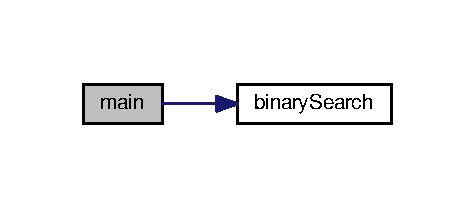
\includegraphics[width=228pt]{BinarySearch_8cpp_ae66f6b31b5ad750f1fe042a706a4e3d4_cgraph}
\end{center}
\end{figure}



%--- End generated contents ---

% Index
\backmatter
\newpage
\phantomsection
\clearemptydoublepage
\addcontentsline{toc}{chapter}{Index}
\printindex

\end{document}
